\documentclass[14pt]{extbook}
\usepackage{multicol, enumerate, enumitem, hyperref, color, soul, setspace, parskip, fancyhdr} %General Packages
\usepackage{amssymb, amsthm, amsmath, bbm, latexsym, units, mathtools} %Math Packages
\everymath{\displaystyle} %All math in Display Style
% Packages with additional options
\usepackage[headsep=0.5cm,headheight=12pt, left=1 in,right= 1 in,top= 1 in,bottom= 1 in]{geometry}
\usepackage[usenames,dvipsnames]{xcolor}
\usepackage{dashrule}  % Package to use the command below to create lines between items
\newcommand{\litem}[1]{\item#1\hspace*{-1cm}\rule{\textwidth}{0.4pt}}
\pagestyle{fancy}
\lhead{Progress Quiz 9}
\chead{}
\rhead{Version A}
\lfoot{8590-6105}
\cfoot{}
\rfoot{Fall 2020}
\begin{document}

\begin{enumerate}
\litem{
Solve the quadratic equation below. Then, choose the intervals that the solutions $x_1$ and $x_2$ belong to, with $x_1 \leq x_2$.\[ 25x^{2} +60 x + 36 = 0 \]\begin{enumerate}[label=\Alph*.]
\item \( x_1 \in [-1.67, -0.62] \text{ and } x_2 \in [-1.37, -1.13] \)
\item \( x_1 \in [-2.71, -2.09] \text{ and } x_2 \in [-0.62, -0.43] \)
\item \( x_1 \in [-30.32, -29.56] \text{ and } x_2 \in [-30.09, -29.82] \)
\item \( x_1 \in [-4.21, -2.61] \text{ and } x_2 \in [-0.5, -0.34] \)
\item \( x_1 \in [-6.1, -5.64] \text{ and } x_2 \in [-0.27, -0.21] \)

\end{enumerate} }
\litem{
Write the equation of the graph presented below in the form $f(x)=ax^2+bx+c$, assuming  $a=1$ or $a=-1$. Then, choose the intervals that $a, b,$ and $c$ belong to.
\begin{center}
    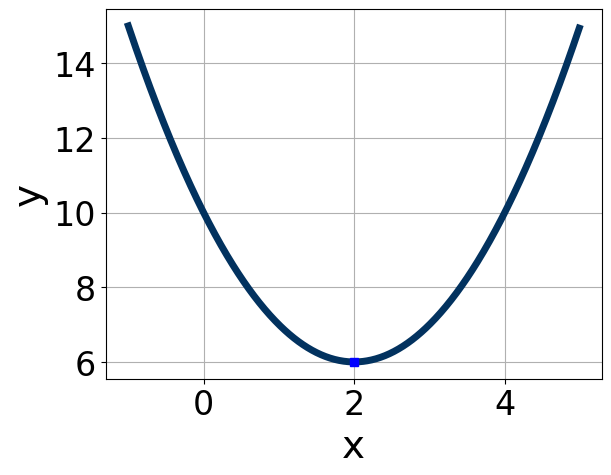
\includegraphics[width=0.5\textwidth]{../Figures/quadraticGraphToEquationA.png}
\end{center}
\begin{enumerate}[label=\Alph*.]
\item \( a \in [-3, 0], \hspace*{5mm} b \in [4, 6], \text{ and } \hspace*{5mm} c \in [-11, -7] \)
\item \( a \in [-3, 0], \hspace*{5mm} b \in [-9, 0], \text{ and } \hspace*{5mm} c \in [1, 8] \)
\item \( a \in [-3, 0], \hspace*{5mm} b \in [-9, 0], \text{ and } \hspace*{5mm} c \in [-11, -7] \)
\item \( a \in [1, 2], \hspace*{5mm} b \in [-9, 0], \text{ and } \hspace*{5mm} c \in [-3, 0] \)
\item \( a \in [1, 2], \hspace*{5mm} b \in [4, 6], \text{ and } \hspace*{5mm} c \in [-3, 0] \)

\end{enumerate} }
\litem{
Solve the quadratic equation below. Then, choose the intervals that the solutions belong to, with $x_1 \leq x_2$ (if they exist).\[ -20x^{2} +8 x + 4 = 0 \]\begin{enumerate}[label=\Alph*.]
\item \( x_1 \in [-0.58, -0.19] \text{ and } x_2 \in [0.54, 0.9] \)
\item \( x_1 \in [-0.91, -0.38] \text{ and } x_2 \in [-0.1, 0.53] \)
\item \( x_1 \in [-13.82, -13.78] \text{ and } x_2 \in [5, 6.26] \)
\item \( x_1 \in [-19.86, -18.94] \text{ and } x_2 \in [19.62, 19.85] \)
\item \( \text{There are no Real solutions.} \)

\end{enumerate} }
\litem{
Write the equation of the graph presented below in the form $f(x)=ax^2+bx+c$, assuming  $a=1$ or $a=-1$. Then, choose the intervals that $a, b,$ and $c$ belong to.
\begin{center}
    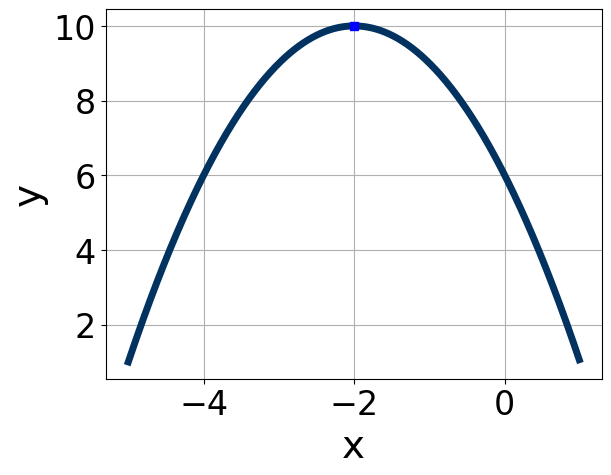
\includegraphics[width=0.5\textwidth]{../Figures/quadraticGraphToEquationCopyA.png}
\end{center}
\begin{enumerate}[label=\Alph*.]
\item \( a \in [-1.3, -0.5], \hspace*{5mm} b \in [-7, 0], \text{ and } \hspace*{5mm} c \in [4, 7] \)
\item \( a \in [0.8, 1.1], \hspace*{5mm} b \in [4, 7], \text{ and } \hspace*{5mm} c \in [12, 15] \)
\item \( a \in [-1.3, -0.5], \hspace*{5mm} b \in [4, 7], \text{ and } \hspace*{5mm} c \in [4, 7] \)
\item \( a \in [-1.3, -0.5], \hspace*{5mm} b \in [4, 7], \text{ and } \hspace*{5mm} c \in [-15, -12] \)
\item \( a \in [0.8, 1.1], \hspace*{5mm} b \in [-7, 0], \text{ and } \hspace*{5mm} c \in [12, 15] \)

\end{enumerate} }
\litem{
Solve the quadratic equation below. Then, choose the intervals that the solutions belong to, with $x_1 \leq x_2$ (if they exist).\[ 14x^{2} -10 x -9 = 0 \]\begin{enumerate}[label=\Alph*.]
\item \( x_1 \in [-0.7, 0.2] \text{ and } x_2 \in [0.9, 1.3] \)
\item \( x_1 \in [-24.7, -22.5] \text{ and } x_2 \in [23.8, 25.2] \)
\item \( x_1 \in [-1.4, -1] \text{ and } x_2 \in [-0.1, 1] \)
\item \( x_1 \in [-7.5, -6.9] \text{ and } x_2 \in [16.5, 17.5] \)
\item \( \text{There are no Real solutions.} \)

\end{enumerate} }
\litem{
Graph the equation below.\[ f(x) = (x-4)^2 - 12 \]\begin{enumerate}[label=\Alph*.]
\begin{multicols}{2}\item 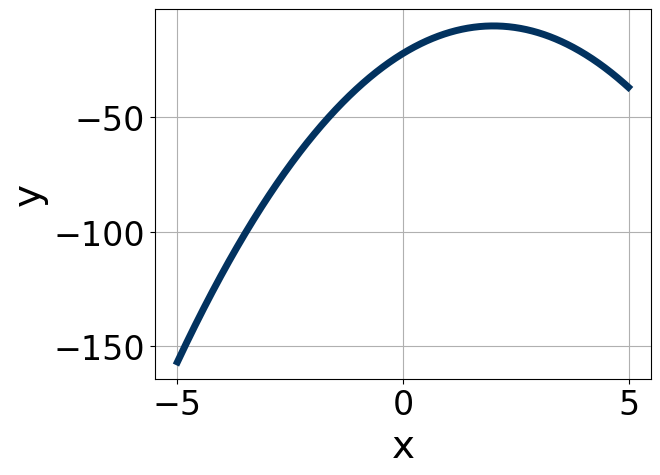
\includegraphics[width = 0.3\textwidth]{../Figures/quadraticEquationToGraphCopyAA.png}\item 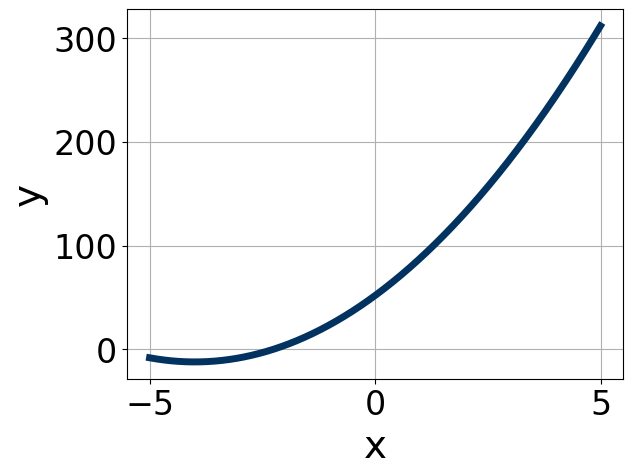
\includegraphics[width = 0.3\textwidth]{../Figures/quadraticEquationToGraphCopyBA.png}\item 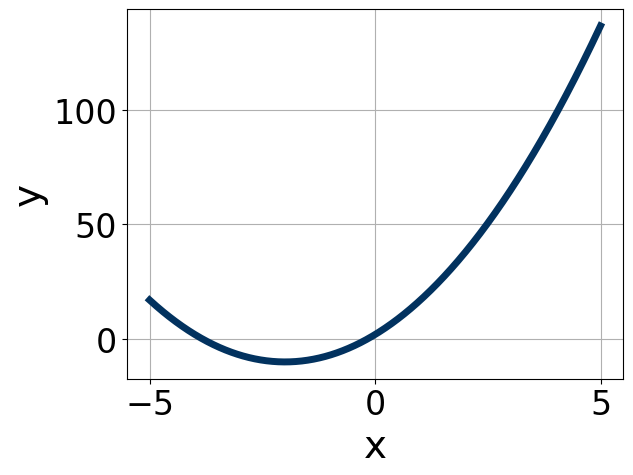
\includegraphics[width = 0.3\textwidth]{../Figures/quadraticEquationToGraphCopyCA.png}\item 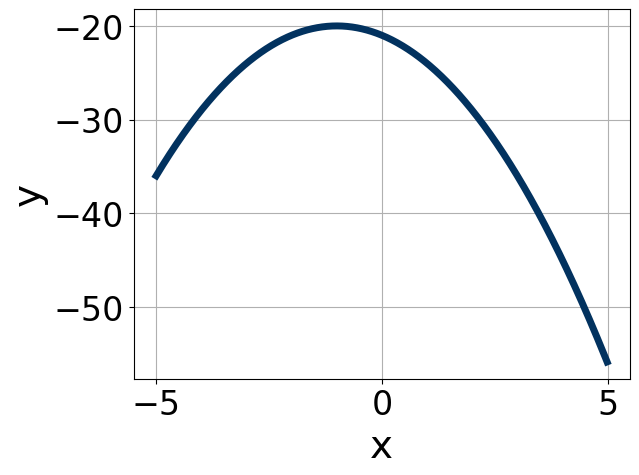
\includegraphics[width = 0.3\textwidth]{../Figures/quadraticEquationToGraphCopyDA.png}\end{multicols}\item None of the above.
\end{enumerate} }
\litem{
Solve the quadratic equation below. Then, choose the intervals that the solutions $x_1$ and $x_2$ belong to, with $x_1 \leq x_2$.\[ 15x^{2} -8 x -16 = 0 \]\begin{enumerate}[label=\Alph*.]
\item \( x_1 \in [-4.74, -3.53] \text{ and } x_2 \in [0.15, 0.57] \)
\item \( x_1 \in [-1.07, -0.65] \text{ and } x_2 \in [1.03, 1.48] \)
\item \( x_1 \in [-0.71, -0.22] \text{ and } x_2 \in [2.57, 2.73] \)
\item \( x_1 \in [-12.42, -11.07] \text{ and } x_2 \in [19.9, 20.12] \)
\item \( x_1 \in [-1.87, -0.88] \text{ and } x_2 \in [0.65, 1.15] \)

\end{enumerate} }
\litem{
Factor the quadratic below. Then, choose the intervals that contain the constants in the form $(ax+b)(cx+d); b \leq d.$\[ 81x^{2} -81 x + 20 \]\begin{enumerate}[label=\Alph*.]
\item \( a \in [1, 2], \hspace*{5mm} b \in [-45, -40], \hspace*{5mm} c \in [0, 2], \text{ and } \hspace*{5mm} d \in [-39, -35] \)
\item \( a \in [27, 30], \hspace*{5mm} b \in [-14, -2], \hspace*{5mm} c \in [3, 7], \text{ and } \hspace*{5mm} d \in [-4, -3] \)
\item \( a \in [4, 12], \hspace*{5mm} b \in [-14, -2], \hspace*{5mm} c \in [8, 13], \text{ and } \hspace*{5mm} d \in [-4, -3] \)
\item \( a \in [3, 4], \hspace*{5mm} b \in [-14, -2], \hspace*{5mm} c \in [27, 28], \text{ and } \hspace*{5mm} d \in [-4, -3] \)
\item \( \text{None of the above.} \)

\end{enumerate} }
\litem{
Factor the quadratic below. Then, choose the intervals that contain the constants in the form $(ax+b)(cx+d); b \leq d.$\[ 36x^{2} +25 x -25 \]\begin{enumerate}[label=\Alph*.]
\item \( a \in [0.1, 2.6], \hspace*{5mm} b \in [-21, -19], \hspace*{5mm} c \in [0.8, 2.4], \text{ and } \hspace*{5mm} d \in [41, 48] \)
\item \( a \in [26.7, 30.7], \hspace*{5mm} b \in [-8, -1], \hspace*{5mm} c \in [0.8, 2.4], \text{ and } \hspace*{5mm} d \in [1, 6] \)
\item \( a \in [7.3, 9.3], \hspace*{5mm} b \in [-8, -1], \hspace*{5mm} c \in [3.7, 6.4], \text{ and } \hspace*{5mm} d \in [1, 6] \)
\item \( a \in [3.6, 4.1], \hspace*{5mm} b \in [-8, -1], \hspace*{5mm} c \in [5.3, 11.9], \text{ and } \hspace*{5mm} d \in [1, 6] \)
\item \( \text{None of the above.} \)

\end{enumerate} }
\litem{
Graph the equation below.\[ f(x) = -(x-1)^2 - 12 \]\begin{enumerate}[label=\Alph*.]
\begin{multicols}{2}\item 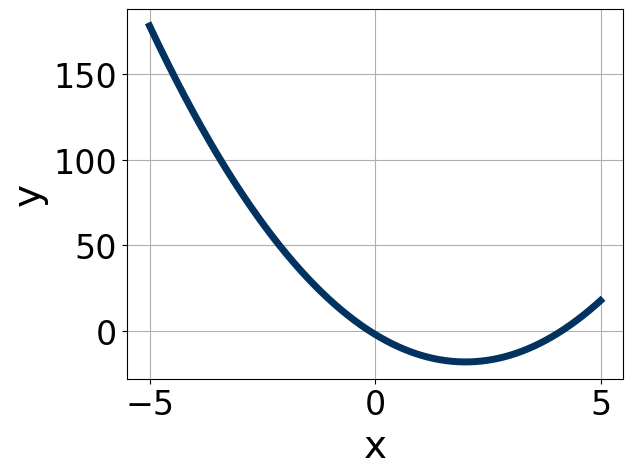
\includegraphics[width = 0.3\textwidth]{../Figures/quadraticEquationToGraphAA.png}\item 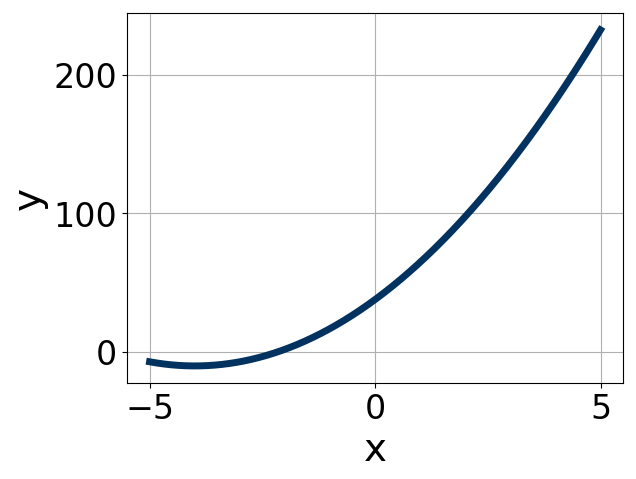
\includegraphics[width = 0.3\textwidth]{../Figures/quadraticEquationToGraphBA.png}\item 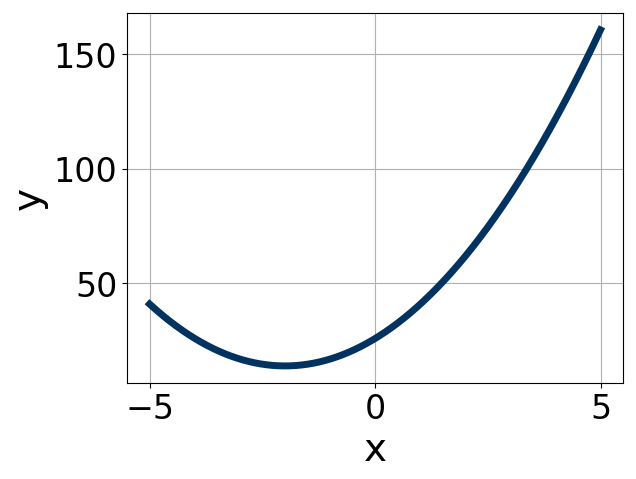
\includegraphics[width = 0.3\textwidth]{../Figures/quadraticEquationToGraphCA.png}\item 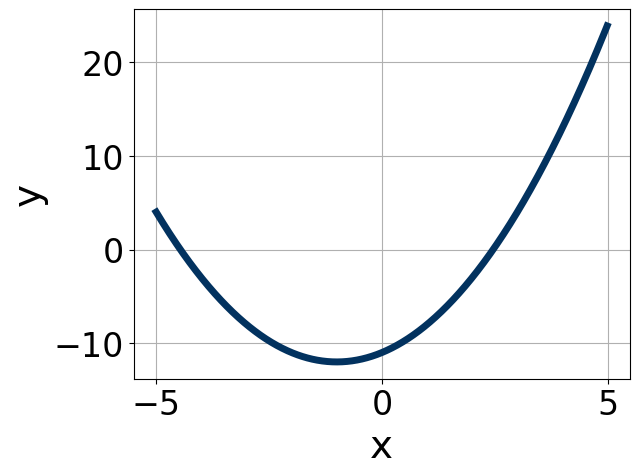
\includegraphics[width = 0.3\textwidth]{../Figures/quadraticEquationToGraphDA.png}\end{multicols}\item None of the above.
\end{enumerate} }
\end{enumerate}

\end{document}